\documentclass{standalone}
\usepackage{graphicx}	
\usepackage{amssymb, amsmath}
\usepackage{color}

\usepackage{tikz}
\usetikzlibrary{intersections, backgrounds}

\definecolor{light}{RGB}{220, 188, 188}
\definecolor{mid}{RGB}{185, 124, 124}
\definecolor{dark}{RGB}{143, 39, 39}
\definecolor{highlight}{RGB}{180, 31, 180}
\definecolor{gray10}{gray}{0.1}
\definecolor{gray20}{gray}{0.2}
\definecolor{gray30}{gray}{0.3}
\definecolor{gray40}{gray}{0.4}
\definecolor{gray60}{gray}{0.6}
\definecolor{gray70}{gray}{0.7}
\definecolor{gray80}{gray}{0.8}
\definecolor{gray90}{gray}{0.9}
\definecolor{gray95}{gray}{0.95}

\begin{document}

\begin{tikzpicture}[scale=0.35, thick]

  \node[] at (-12, 5) {
\includegraphics[width=4.9cm]{differential_volumes_before.pdf}};
  \draw [rounded corners=2pt, color=black] (-5, 0) rectangle +(-14, 10);
  \node at (-12, -1) { $X = \mathbb{R}^{2}$ };
  \node at (-12, 11) { $\mathbb{P} [ A ] = \int_{A} \mathrm{d} x \, \pi(x)$ };
  
  %\fill [fill=light, text=white] (-14.1, 3.5) circle (2);
  \node[text=white] at (-14.1, 3.5) { $A$ };
  
  \node at (0, -1) { $g: X \rightarrow Y$ };
  
  \node[] at (12, 5) {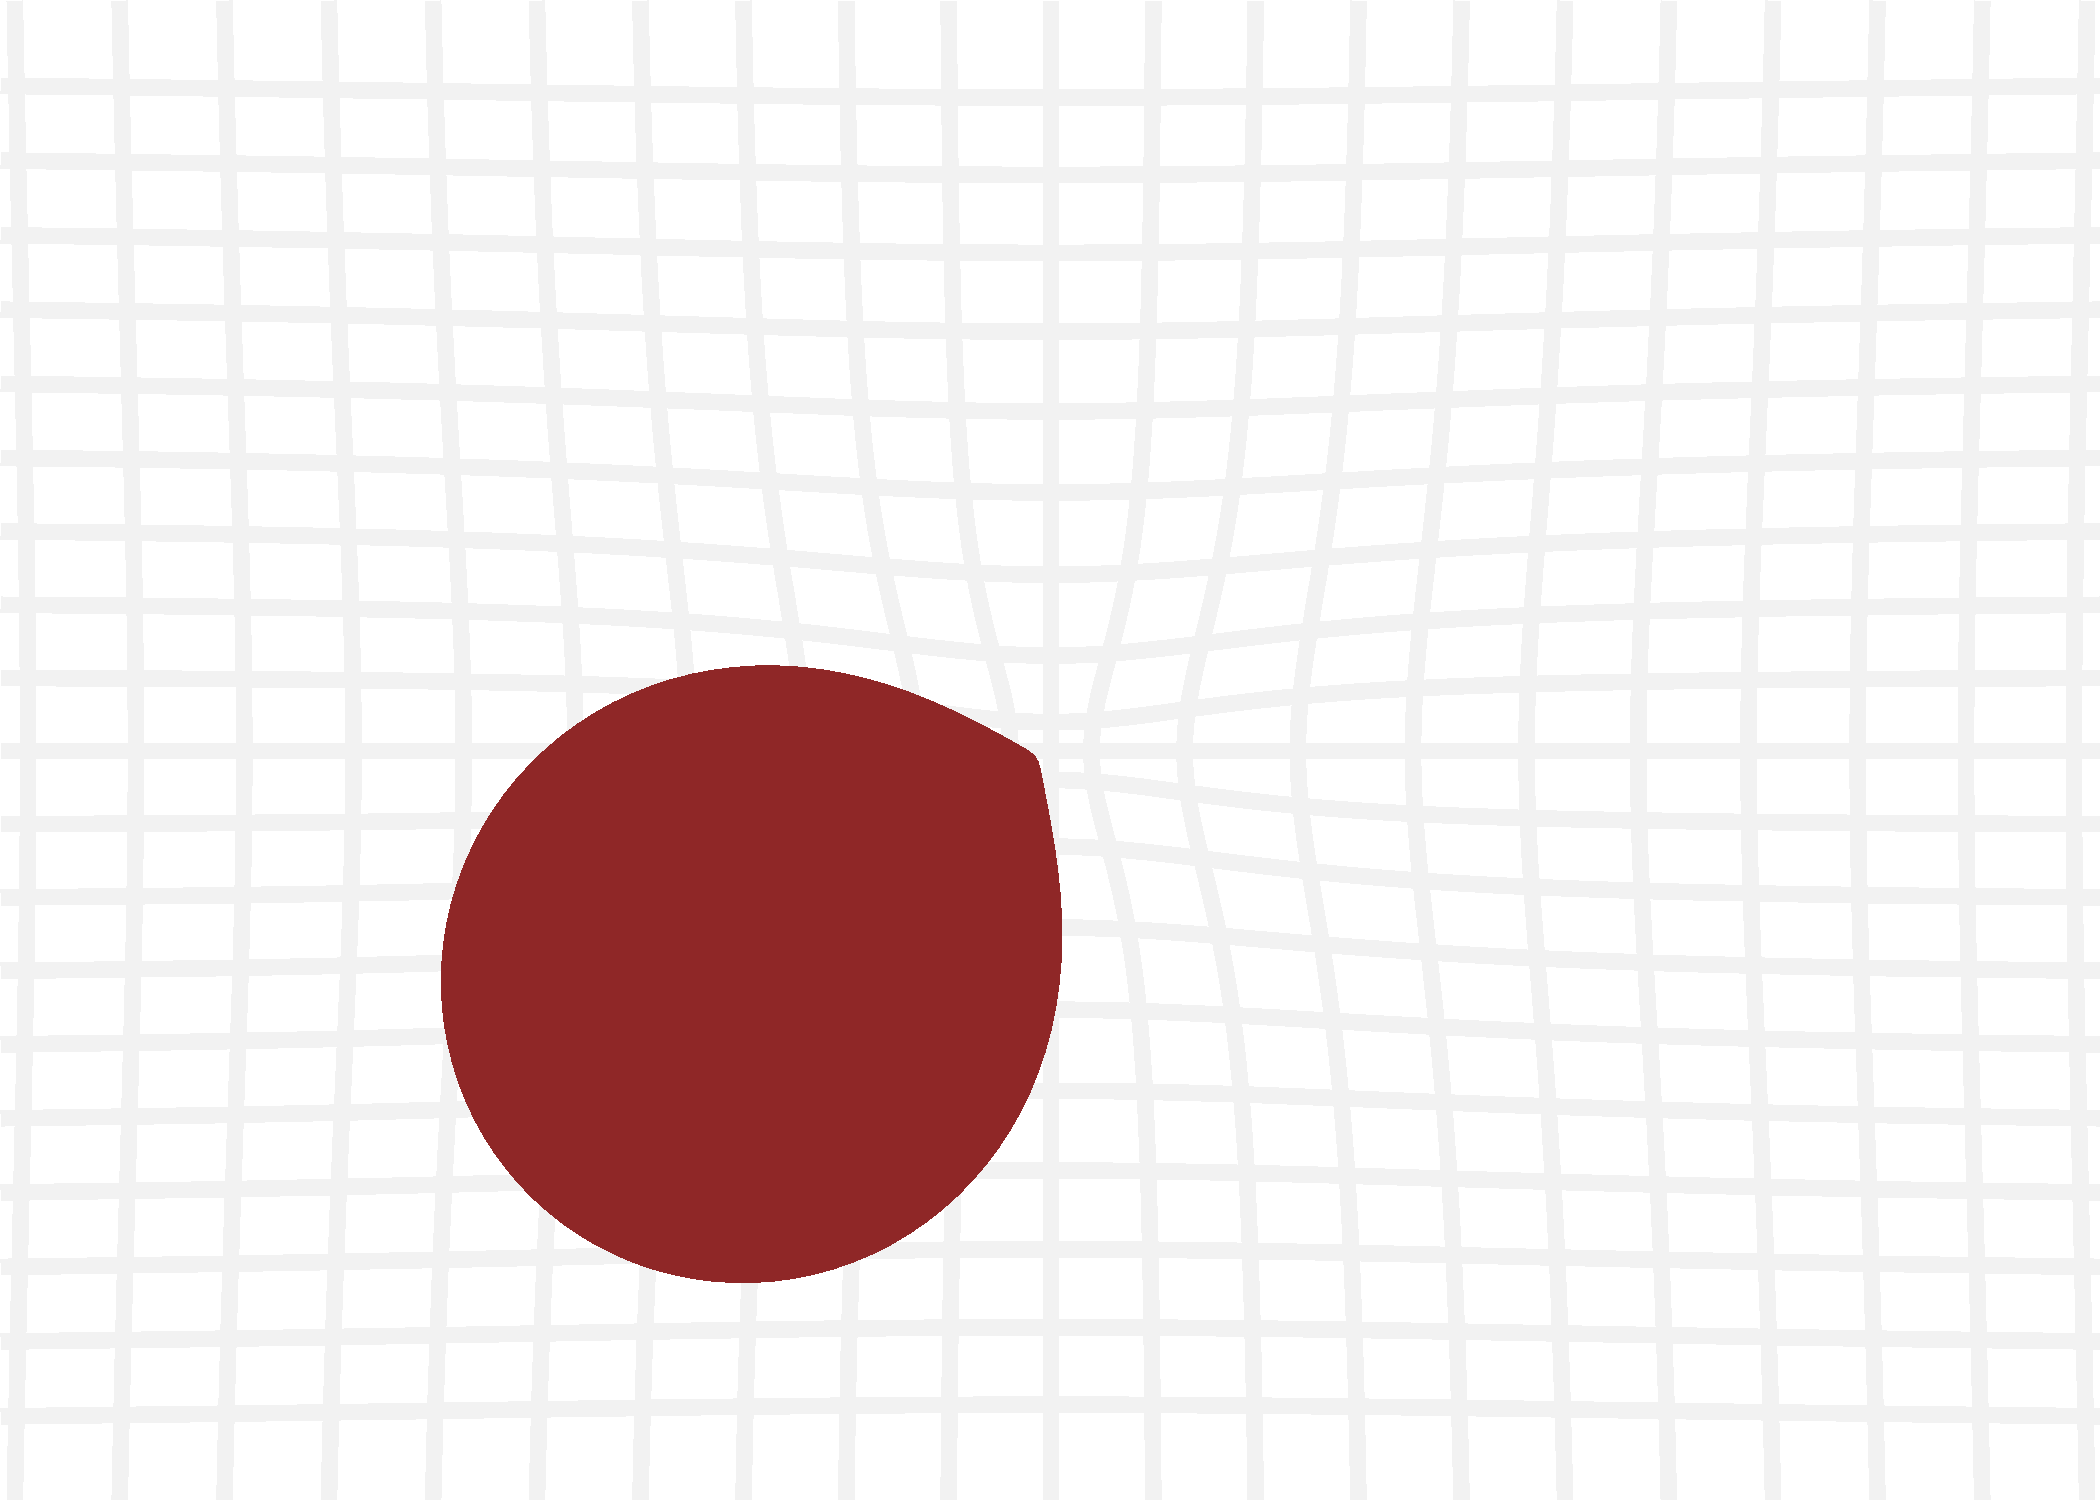
\includegraphics[width=4.9cm]{differential_volumes_after.pdf}};
  \draw [rounded corners=2pt, color=black] (5, 0) rectangle +(14, 10);
  \node at (12, -1) { $Y = \mathbb{R}^{2}$ };
  \node at (12, 11) { $\mathbb{P} [ g(A) ] = \int_{g(A)} \mathrm{d} y \, \pi_{*} (y)$ };
  
  \node[text=white] at (9.9, 3.5) { $g(A)$ };
  
\end{tikzpicture}

\end{document}  